\section{Calorimeter Noise simulation}
\label{sc:CaloNoise}

Random fluctuations in electronics noise can be a source of a small amount of missing energy. Therefore, the first step
in making comparisons between Monte Carlo and data is to look at the detector noise simulation. Figures~\ref{fig:RecHitE_ECAL},
\ref{fig:RecHitE_HCAL_1}, and \ref{fig:RecHitE_HCAL_2} show the comparison between RecHit energy distributions in noise-only
Monte Carlo and zero bias data.

\begin{figure}[h!]
 \centering
 \begin{tabular}{ll}
  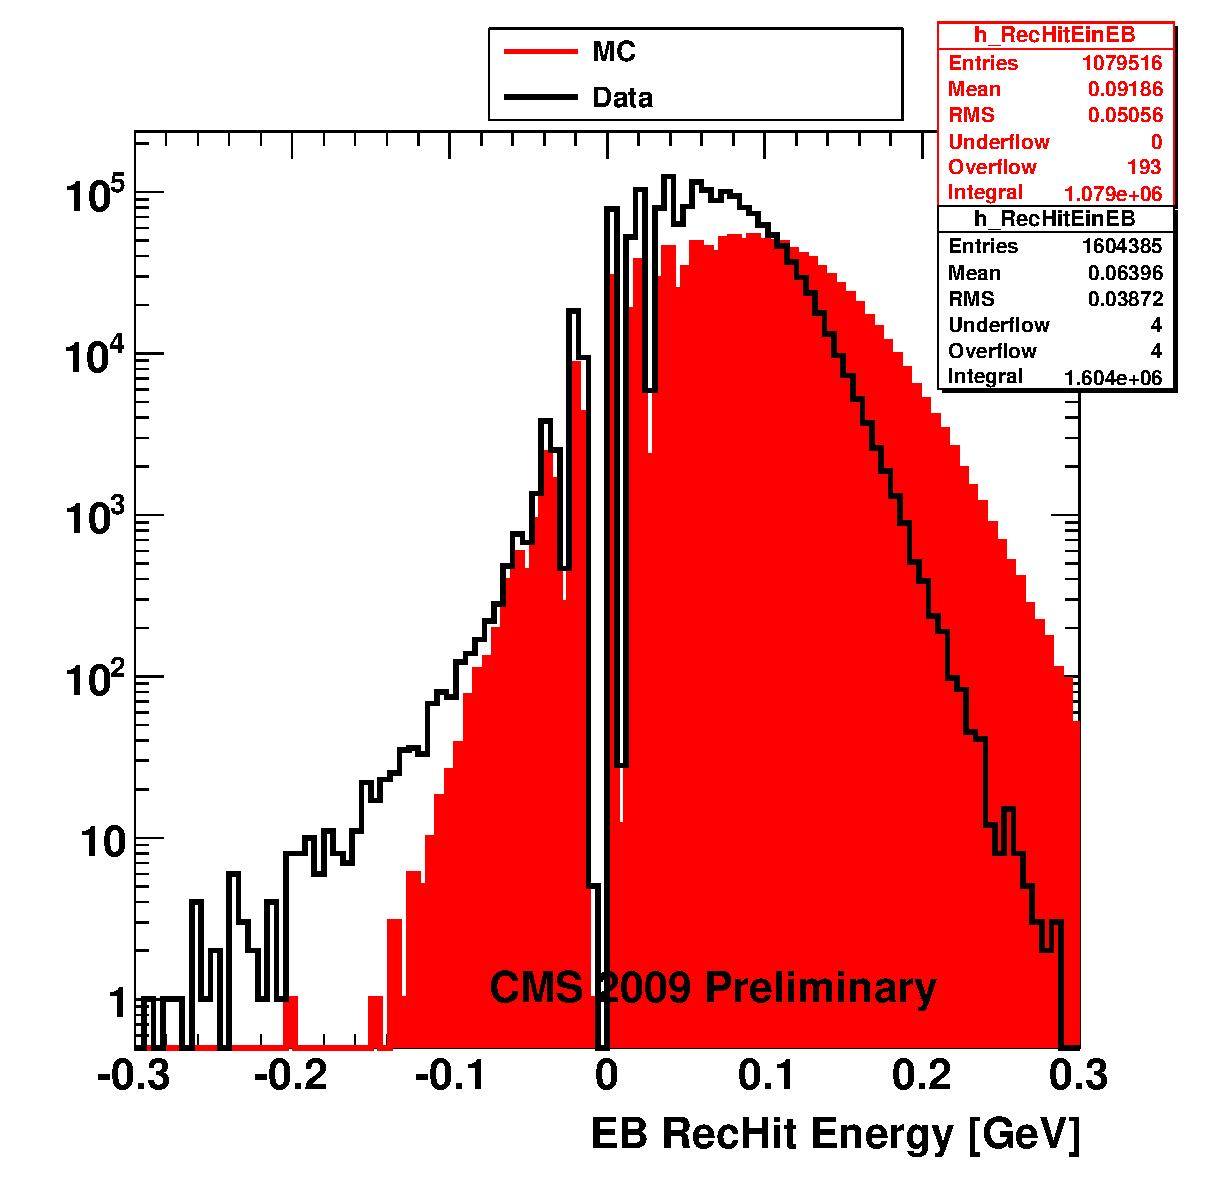
\includegraphics[width=0.33\textwidth]{plots_CaloNoise/h_RecHitEinEB.eps} &
  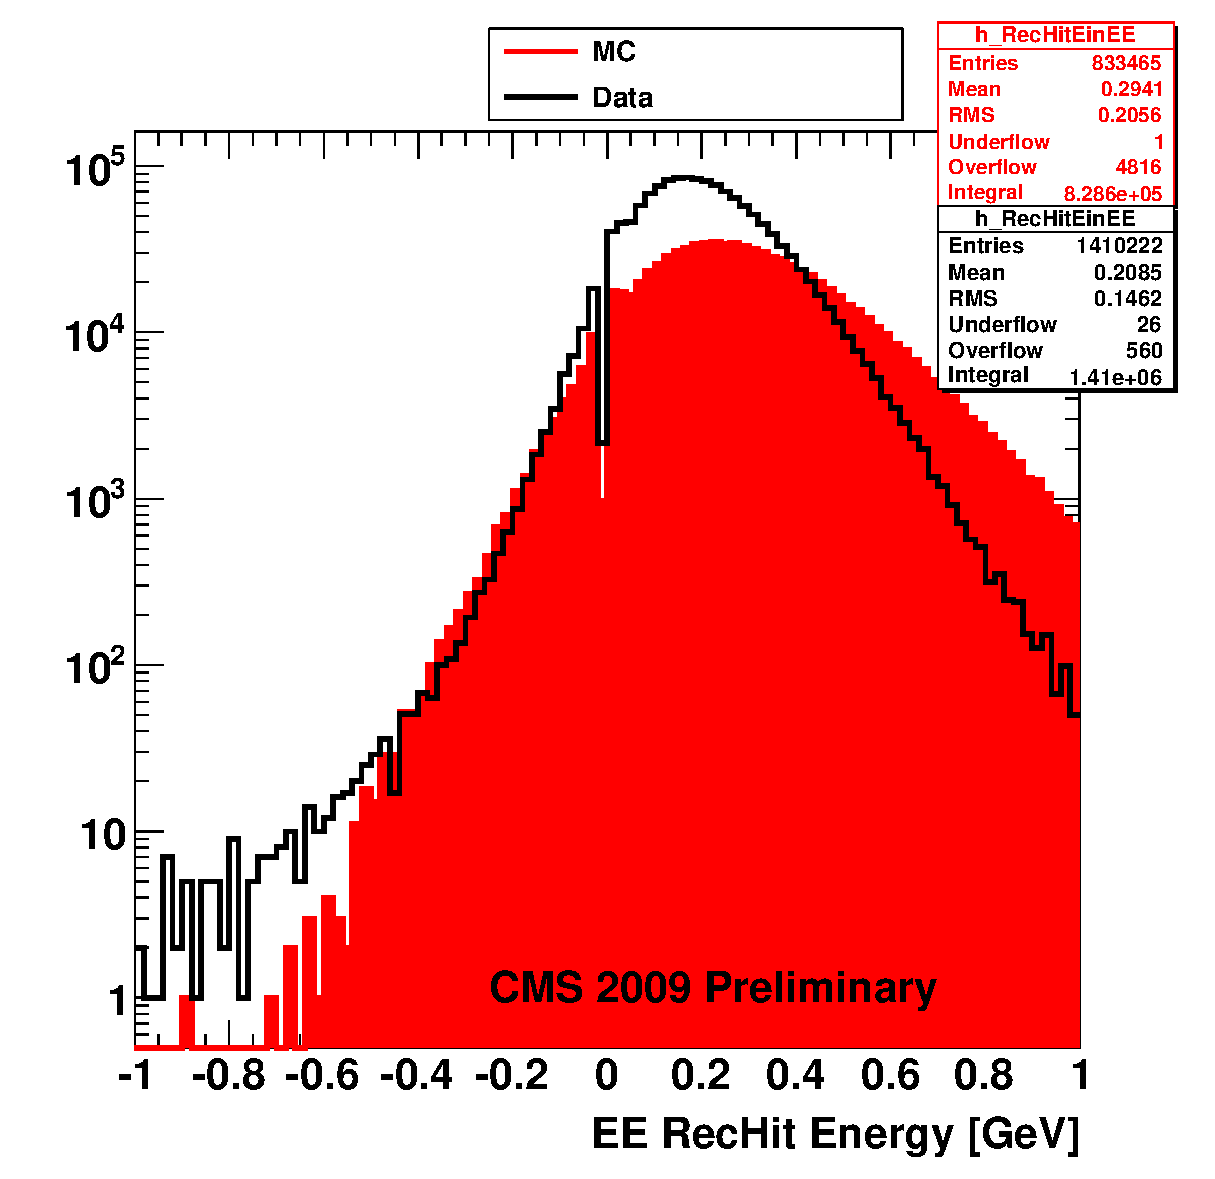
\includegraphics[width=0.33\textwidth]{plots_CaloNoise/h_RecHitEinEE.eps} \\
 \end{tabular}
 \caption{\small Comparison of the RecHit energy distributions in EB and EE for 2000 events in noise-only Monte Carlo
          and zero bias data for run 123596.\label{fig:RecHitE_ECAL}}
\end{figure}

\begin{figure}[h!]
 \centering
 \begin{tabular}{lll}
  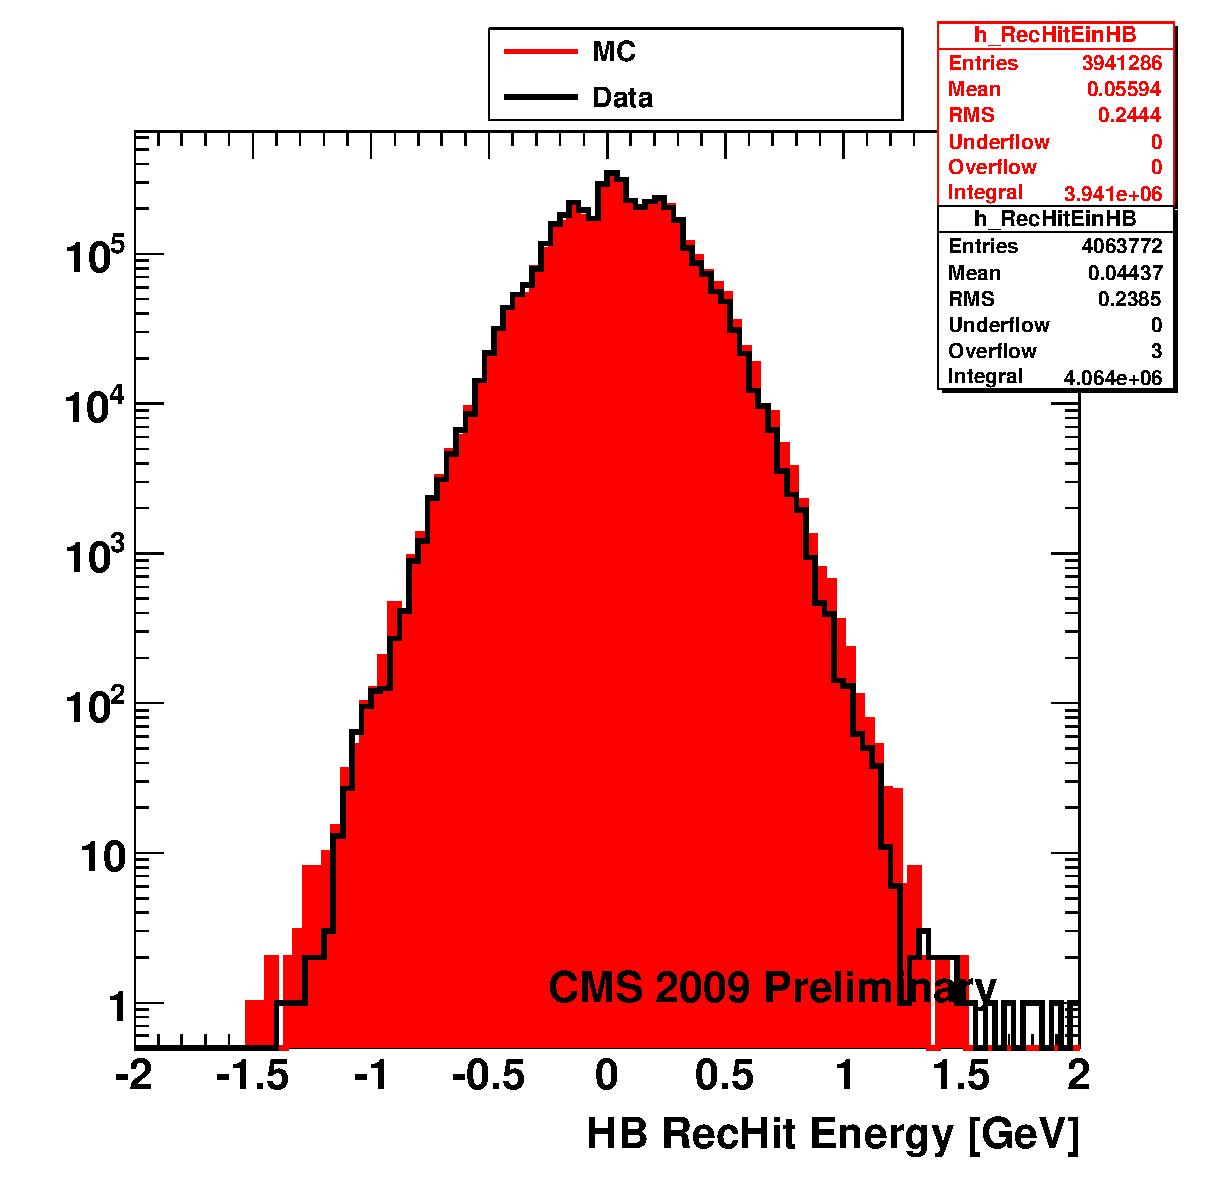
\includegraphics[width=0.33\textwidth]{plots_CaloNoise/h_RecHitEinHB.eps} &
  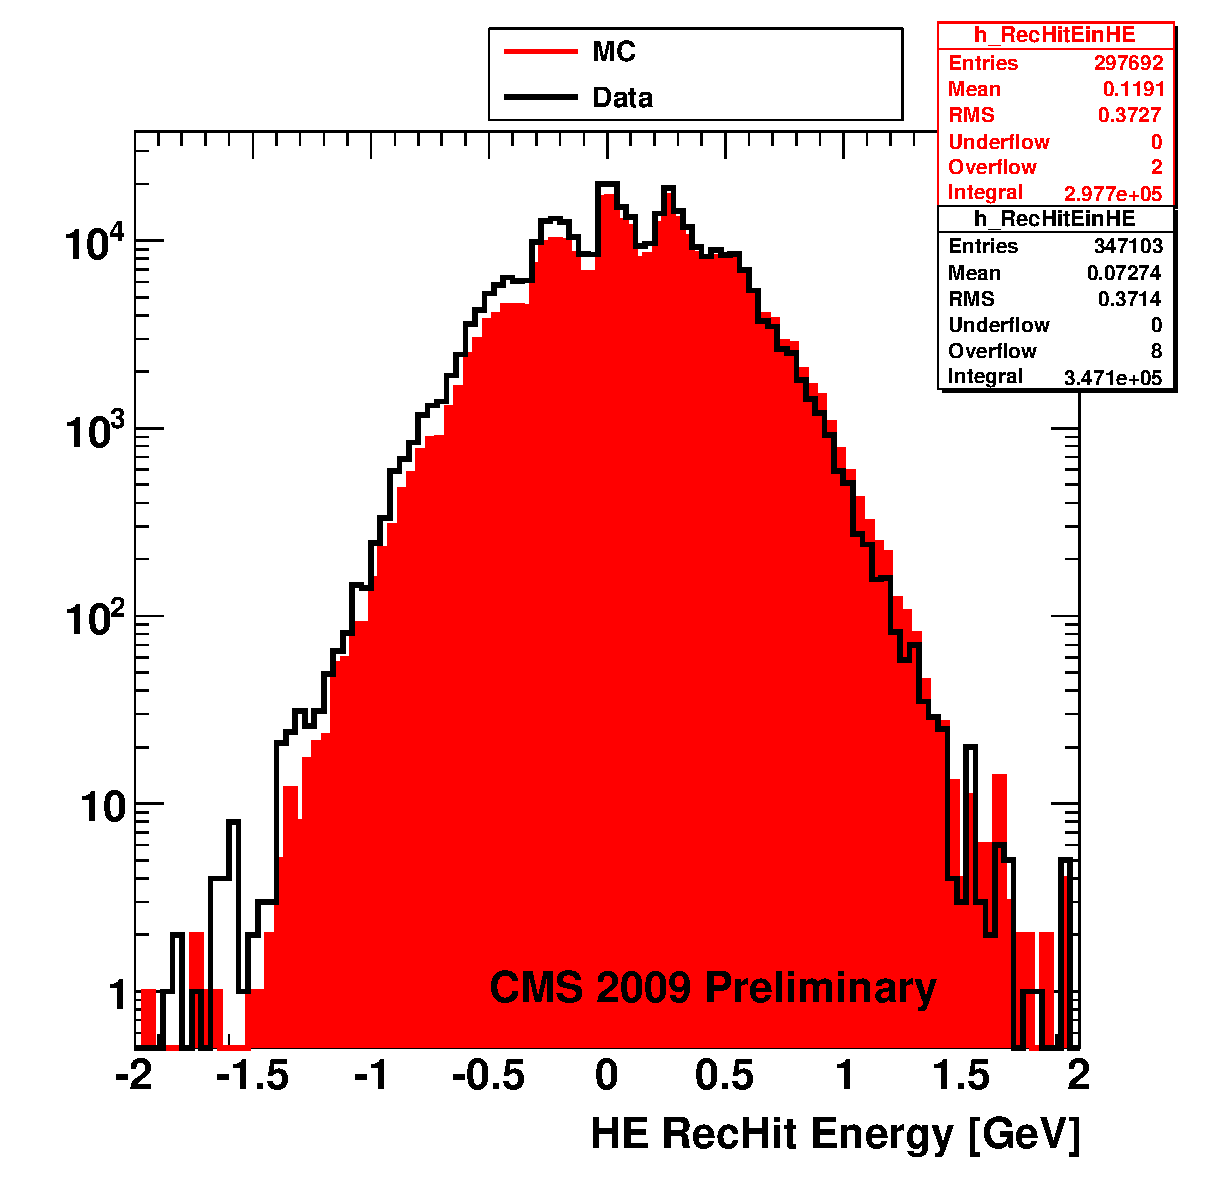
\includegraphics[width=0.33\textwidth]{plots_CaloNoise/h_RecHitEinHE.eps} &
  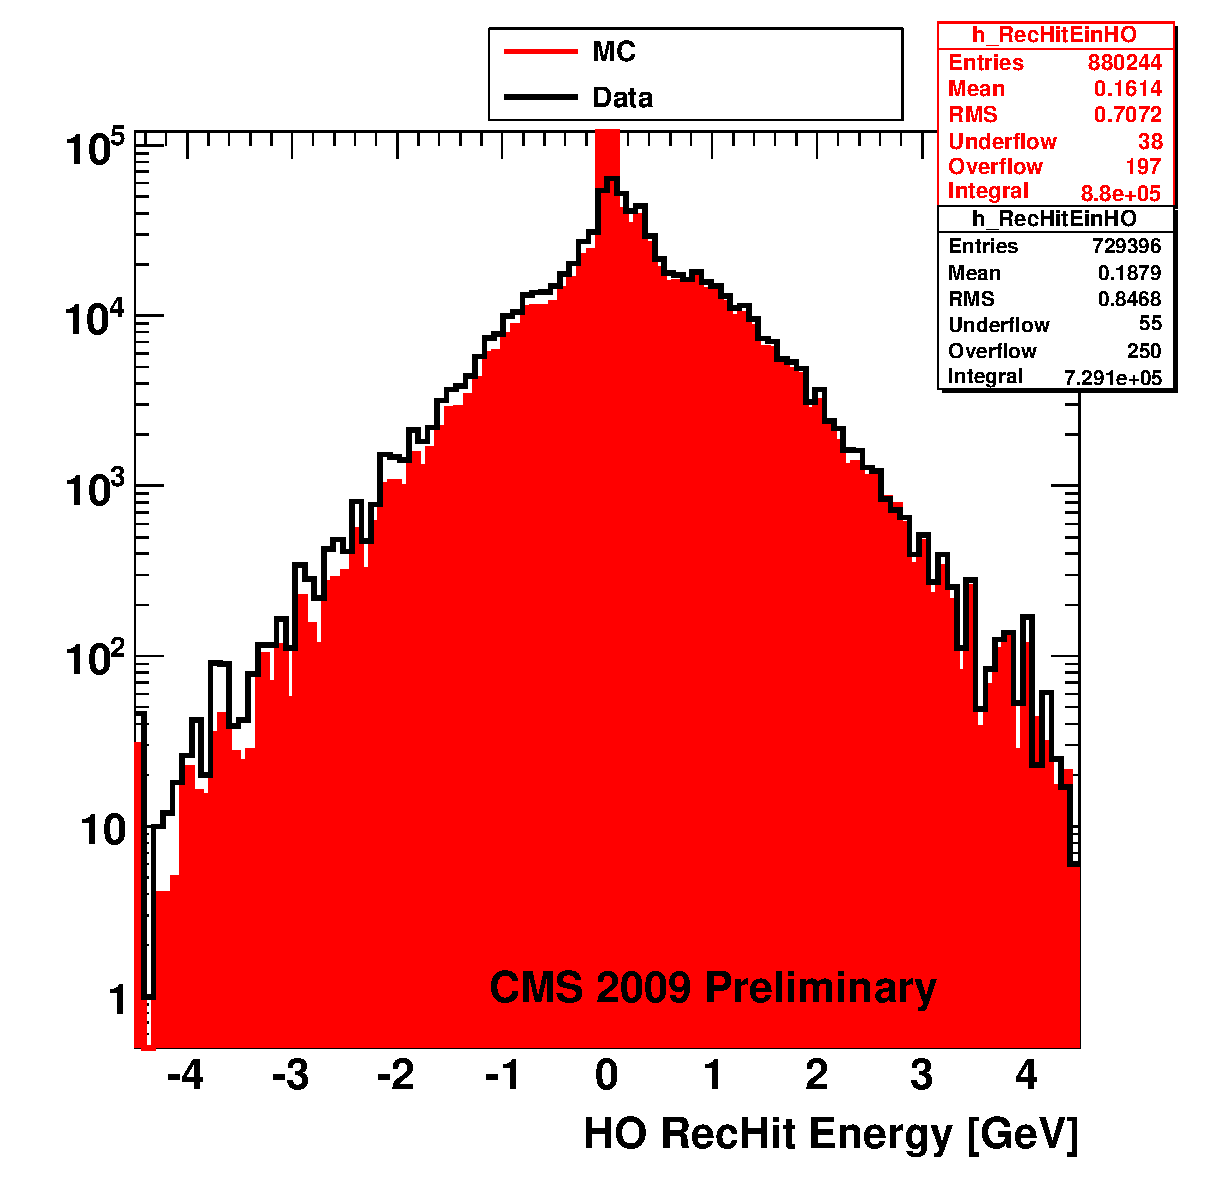
\includegraphics[width=0.33\textwidth]{plots_CaloNoise/h_RecHitEinHO.eps} \\
 \end{tabular}
 \caption{\small Comparison of the RecHit energy distributions in HB, HE, and HO for 2000 events in noise-only Monte Carlo
          and zero bias data for run 123596.\label{fig:RecHitE_HCAL_1}}
\end{figure}

\begin{figure}[h!]
 \centering
 \begin{tabular}{ll}
  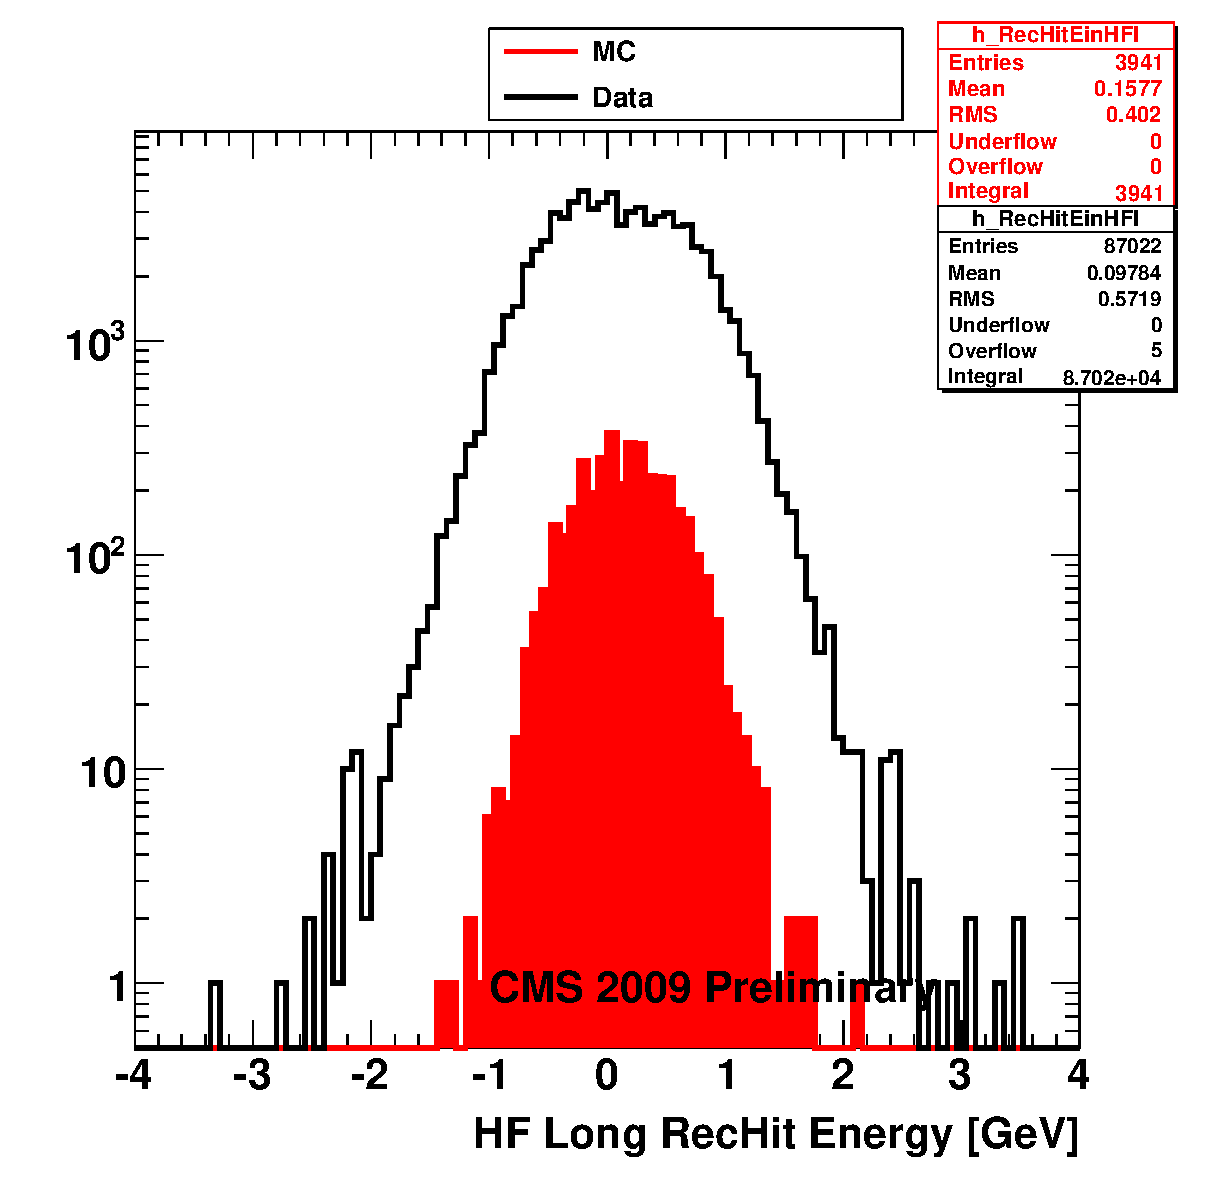
\includegraphics[width=0.33\textwidth]{plots_CaloNoise/h_RecHitEinHFl.eps} &
  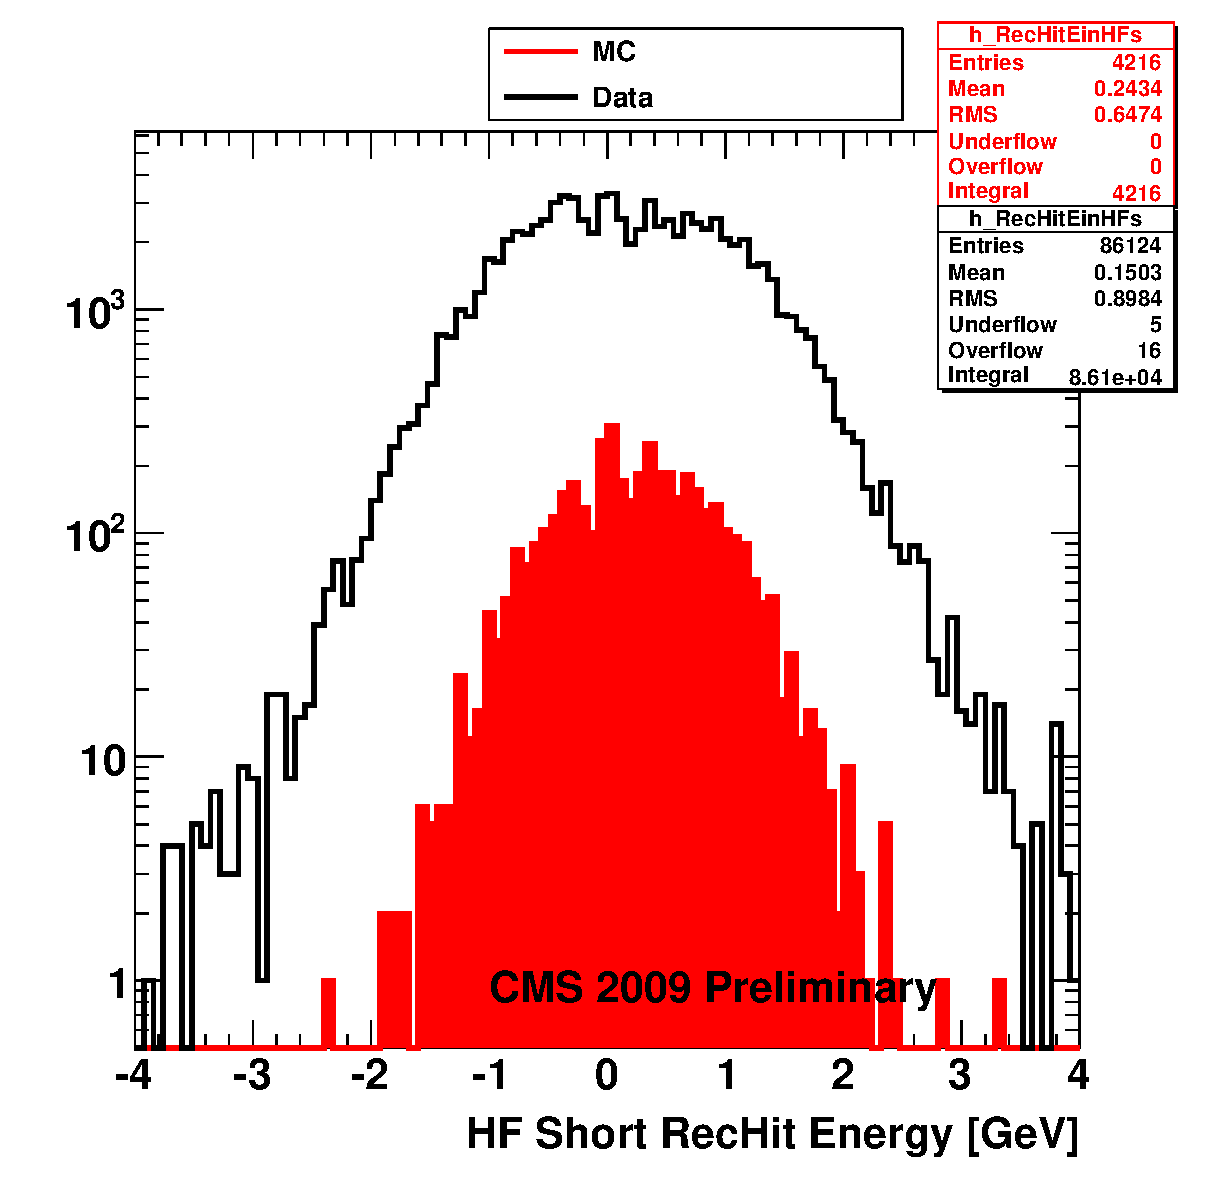
\includegraphics[width=0.33\textwidth]{plots_CaloNoise/h_RecHitEinHFs.eps} \\
 \end{tabular}
 \caption{\small Comparison of the RecHit energy distributions in HF for 2000 events in noise-only Monte Carlo
          and zero bias data for run 123596.\label{fig:RecHitE_HCAL_2}}
\end{figure}